\documentclass[a4paper, 12pt, table]{scrartcl}

% Use Hungarian Locale
\usepackage[magyar]{babel}

% Inputs
% Link between TeX and lua files
\usepackage{pyluatex}

% \begin{noindent}
\begin{python}
import sympy as sp
from sympy.printing.latex import print_latex
from sympy import latex
from python.calc import calculate

V = calculate({
    "code": {
        1: 1,
        2: 1,
        3: 4,
        4: 2,
    },
    "name": "Sándor Tibor",
    "neptun": "C7XUDE"
})

N = V["numeric"]
P = V["parametric"]

from python.helper import get_printer, print_SI_direct, print_matrix, prin_TeX, my_latex

print_SI_var = get_printer(V)
\end{python}
% \end{noindent}

\usepackage{xargs}

\newcommand{\pv}[1]{\py{V["#1"]}}
\newcommand{\pvec}[2]{\py{V["#1"][#2]}}
\newcommand{\pmat}[3]{\py{V["#1"][#2, #3]}}

\newcommandx{\sipv}[3][3=]{\pyc{print_SI_var({ "name":"#1", "unit":"#2", "dec":"#3" })}}
\newcommandx{\sipvec}[4][4=]{\pyc{print_SI_direct({ "value":V["#1"][#2], "unit":"#3", "dec":"#4" })}}
\newcommandx{\sipmat}[5][5=]{\pyc{print_SI_direct({ "value":V["#1"][#2, #3], "unit":"#4", "dec":"#5" })}}

% Figure and other imports
\usepackage{pdfpages}
\usepackage{standalone}

% Actual page layout
\usepackage[
  margin=20mm,
  footskip=16mm,
  headheight=20mm,
  % showframe
]{geometry}
\usepackage{lastpage}
\usepackage[
  colorlinks=true,
  allcolors=red!40!black,
]{hyperref}

\setlength\parindent{0em}
\setlength\parskip{.30em}

\usepackage[
  headsepline=1mm,
  footsepline=1mm,
]{scrlayer-scrpage}
\pagestyle{scrheadings}
\setkomafont{pageheadfoot}{\color{gray}}

\ModifyLayer[addvoffset=-2mm]{scrheadings.foot.above.line}
\cfoot{\thepage\ / \pageref{LastPage}}
\ihead{BMEGEMMBXVE, 2. Házi Feladat}
\ohead{%
  
\includegraphics[height = 12px]{static/signature.pdf}
  \py{V["name"]},
  \py{V["neptun"]}
}

\usepackage{caption}
\setkomafont{disposition}{\color{red!40!black}\bfseries\sffamily}
\setkomafont{captionlabel}{\color{red!40!black}\bfseries\sffamily}

% Math related stuff goes here
\usepackage{amsmath}
\usepackage{nccmath}
\usepackage{amssymb}
\usepackage{fontspec}
\usepackage{unicode-math}

% Set font to my liking
\setmainfont{TeX Gyre Termes}
\setsansfont[Scale=MatchUppercase]{TeX Gyre Heros}
\setmathfont{Asana Math}

% Variable printing according to Hungarian standards
\usepackage{icomma}
\usepackage{siunitx}
\sisetup{
  per-mode = symbol,
  locale=DE
}

% Slanted frac
\usepackage{xfrac}
% Derivatives
\usepackage{derivative}

% Math custom commands
\newcommand\iu{\mathbf{j}}
\newcommand{\rvec}[1]{\mathbfit{#1}}
\newcommand{\uvec}[1]{\widehat{\mathbfit{#1}}}
\newcommand{\rmat}[1]{\mathbf{#1}}
\newcommand{\spec}[1]{\mathfrak{#1}}

% Operator like commands
\DeclareMathOperator\atann{atan2}

% Switching between SI modes
\newcommand{\sifigures}[1]{\sisetup{round-mode=figures, round-precision=#1}}
\newcommand{\siplaces}[1]{\sisetup{round-mode=places, round-precision=#1}}
\newcommand{\sisci}{\sisetup{exponent-mode = scientific}}
\newcommand{\sifix}{\sisetup{exponent-mode = fixed}}

% Framed equations
\usepackage{mdframed}
% \begin{noindent}
\newenvironment{myframe}{%
\begin{mdframed}[%
backgroundcolor=gray!10,%
linecolor=red!40!black,%
linewidth=1mm,%
topline=false,%
rightline=false,%
bottomline=false,%
]\useshortskip}{\end{mdframed}}
% \end{noindent}

\usepackage{tikz}
\usepackage{pgfplots}
\pgfplotsset{compat=1.18, width=16cm, height=8.33cm}
\usepgfplotslibrary{fillbetween}
\pgfkeys{/pgf/number format/use comma}
\pgfkeys{/pgf/number format/1000 sep={\,}}
\pgfplotsset{%
  % xmin=0,xmax=\lv{c}*1.05,
  every major tick/.style = {gray, semithick},
  axis x line=center,  axis y line=center,
  enlarge y limits=.05,
  axis line style={-to, thick},
  grid=both,
  grid style={line width=.1pt, draw=gray!20},
  major grid style={line width=.2pt,draw=gray!80},
  scaled y ticks=false,
}
\usetikzlibrary{
  calc,
  angles,
  quotes,
  backgrounds,
  patterns,
  arrows,
  arrows.meta,
  positioning,
  intersections,
  shapes.geometric,
}

\tikzset{
  dot/.style = {
      circle,
      fill=red!40!gray,
      minimum size=#1,
      draw=black,
      inner sep=0pt, outer sep=0pt,
      very thick,
    },
  dot/.default = 7pt,
  gdot/.style = {
      dot=#1,
      fill=white
    },
  gdot/.default = 7pt,
  dim/.style = {
      latex-latex,
      draw=teal,
      ultra thick
    },
  joint/.style = {
      circle,
      draw=black,
      ultra thick,
      fill=cyan!20,
      minimum size=6.5mm,
      inner sep=0,
    },
  square/.style = {
      regular polygon,
      regular polygon sides=4
    },
  rod/.style = {
      rectangle,
      draw=black,
      minimum height=6mm,
      minimum width=6mm,
      fill=yellow!25,
      ultra thick,
      midway,
      outer sep=0,
    },
}

% Other included packages go here
\usepackage{tabto}
\usepackage{multicol}
\usepackage{xcolor}
\usepackage{float}
\usepackage{array}

% Column type for fixed matrix cols
\newcolumntype{x}[1]{>{\centering\arraybackslash\hspace{0pt}}p{#1}}
\newcolumntype{X}[1]{>{$}x{#1}<{$}}


% code: 1142
\begin{document}

\AddToShipoutPictureFG*{
  \setmainfont{Latin Modern Roman}
  \setmathfont{Latin Modern Math}
  \put(12cm,27.33cm){
    \makebox(7.5cm,1cm){
      \hfill \pv{name}
    }
  }
  \put(12cm,26.67cm){
    \makebox(7.5cm,1cm){
      \hfill \pv{neptun}
    }
  }
  \put(15.45cm,26cm){
    \makebox(7.5cm,1cm){
      \hfill 
\includegraphics[height=5mm]{./static/signature.pdf} \hfill
    }
  }

  \put(8.7cm,25.05cm){
    \makebox(17mm,0){\pvec{code}{1}}
    \makebox(12mm,0){\pvec{code}{2}}
    \makebox(15mm,0){\pvec{code}{3}}
    \makebox(12mm,0){\pvec{code}{4}}
  }

  \newcommand\com{\centering}
  \put(18.5mm, 32mm){
    \def\w{28mm}
    \makebox(\w,0){\com{}\pyc{prin_TeX(V["f"]["a"][0], "", "4")}}
    \makebox(\w,0){\com{}\pyc{prin_TeX(V["f"]["a"][1], "", "4")}}
    \makebox(\w,0){\com{}\pyc{prin_TeX(V["f"]["a"][2], "", "4")}}
    \makebox(\w,0){\com{}\pyc{prin_TeX(V["f"]["b"][0], "", "4")}}
    \makebox(\w,0){\com{}\pyc{prin_TeX(V["f"]["b"][1], "", "4")}}
    \makebox(\w,0){\com{}\pyc{prin_TeX(V["f"]["b"][2], "", "4")}}
  }
  \put(18.5mm, 18mm){
    \def\w{28mm}
    \makebox(\w,0){\com{}\pyc{prin_TeX(V["f"]["c"][0], "", "4")}}
    \makebox(\w,0){\com{}\pyc{prin_TeX(V["f"]["c"][1], "", "4")}}
    \makebox(\w,0){\com{}\pyc{prin_TeX(V["f"]["c"][2], "", "4")}}
    \makebox(\w,0){\com{}\pyc{prin_TeX(V["f"]["d"][0], "", "4")}}
    \makebox(\w,0){\com{}\pyc{prin_TeX(V["f"]["d"][1], "", "4")}}
    \makebox(\w,0){\com{}\pyc{prin_TeX(V["f"]["d"][2], "", "4")}}
  }
}
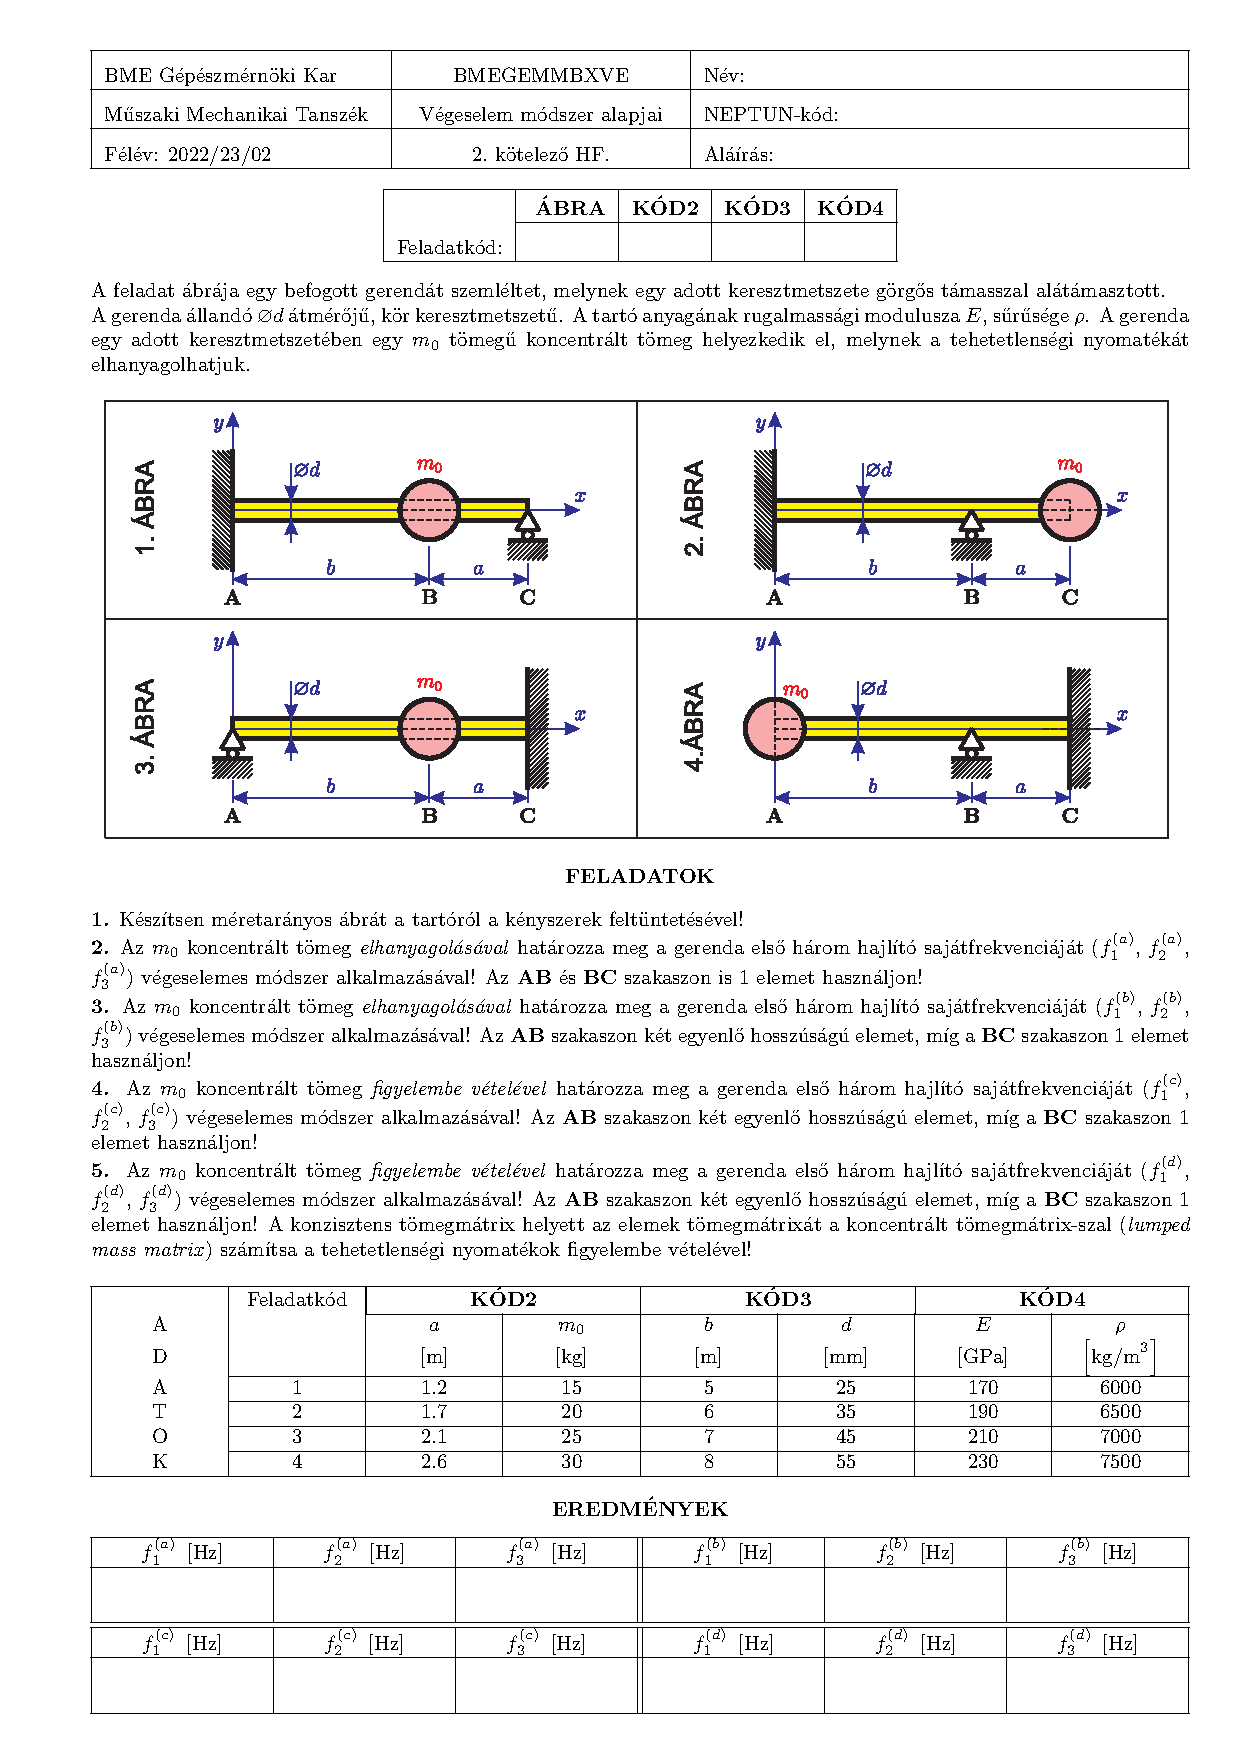
\includepdf[
  pages=-,
  scale=.95,
  pagecommand=\thispagestyle{scrheadings}
]{static/titlepage.pdf}
\setmainfont{TeX Gyre Termes}
\setmathfont{Asana Math}

\allowdisplaybreaks

\def\a{{(a)}}
\def\b{{(b)}}
\def\c{{(c)}}
\def\d{{(d)}}

\section{Méretarányos ábra}

A feladatkódom (\texttt{\pvec{code}{1}\pvec{code}{2}\pvec{code}{3}\pvec{code}{4}})
alapján a szerkezetet jellemző adatok:
\begin{multicols}{2}
  \begin{itemize}
    \item $a = \sipv{a}{m}$,
    \item $b = \sipv{b}{m}$,
    \item $d = \sipv{d}{m}$,

    \item $m_0 = \sipv{m}{kg}$,
    \item $\siplaces{1}\sisci{}E = \sipv{E}{Pa}$,
    \item $\rho = \sipv{rho}{kg/m^3}$.
  \end{itemize}
\end{multicols}

A megadott adatok alapján a szerkezetről készített méretarányos vázlat az
\ref{fig:construction}. ábrán látható. A lapon mért $\SI{1}{cm}$ távolság
a valóságban $\SI{1}{m}$-nek felel meg.

\begin{figure}[H]
  \centering
  \includestandalone{construction}
  \caption{Méretarányos ábra a tartóról}
  \label{fig:construction}
\end{figure}

Az elemek általános geometriai jellemzői:
\begin{itemize}
  \sisci
  \sifigures{4}
  \item $A\phantom{I}\hspace{-1.5mm} = \sipv{A}{m^2}$,
  \item $I\phantom{A}\hspace{-1.5mm} = \sipv{I}{m^4}$,
\end{itemize}

\section{2 elemes modell a koncentrált tömeg elhanyagolásával}

\subsection{Általános adatok}

Jelen feladatrészben a VEM modellünk két elemből és három csomópontból áll.
A csomópontok koordinátáit az \ref{fig:dot-numbering-a}. táblázat tartalmazza.
\begin{table}[H]
  \caption{A csomópontok koordinátái}
  \centering
  \begin{tabular}{|c *{2}{|| X{15mm} | X{15mm} }|}
    \hline
    Csp. & x     & y & x \, [\mathrm{mm}] & y \, [\mathrm{mm}] \\ \hline\hline
    $1$  & 0     & 0 & 0                  & 0                  \\ \hline
    $2$  & b     & 0 & \sipv{b}{}         & 0                  \\ \hline
    $3$  & b + a & 0 & \sipv{c}{}         & 0                  \\ \hline
  \end{tabular}
  \label{fig:dot-numbering-a}
\end{table}

Az egyes elemekhez tartozó csomópontokat, valamint a gerendák hosszát a
\ref{fig:beam-numbering-a}. táblázat foglalja össze.
\begin{table}[H]
  \caption{Elem – csomópont összerendelések}
  \centering
  \begin{tabular}{|c || c | c | c|}
    \hline
    Elem. & 1. csp & 2. csp & $L$ \\ \hline \hline
    $1$   & $1$    & $2$    & $b$ \\ \hline
    $2$   & $2$    & $3$    & $a$ \\ \hline
  \end{tabular}
  \label{fig:beam-numbering-a}
\end{table}

\subsection{A globális merevségi mátrix}

Határozzuk meg először az egyes elemekhez tartozó merevségi mátrixokat. Egy
ilyen mátrix síkbeli gerendák esetén az alábbi alakot veszi fel:
\begin{myframe}
  \begin{equation}
    \rmat K_i
    = \frac{I_i E_i}{L_i}
    \begin{bmatrix}
      12    & 6 L_i     & -12    & 6 L_i     \\
      6 L_i & 4 {L_i}^2 & -6 L_i & 2 {L_i}^2 \\
      -12   & -6 L_i    & -2     & -6 L_i    \\
      6 L_i & 2 {L_i}^2 & -6 L_i & 4 {L_i}^2 \\
    \end{bmatrix}
    \text.
    \label{eq:Ki-base}
  \end{equation}
\end{myframe}

Az elemi merevségi mátrixok numerikusan:
\begin{myframe}
  \begin{align}
    \siplaces{4}
    \sifix{}
    \rmat K_1^\a = \left[
      \begin{array}{*{8}{X{2cm}}}
        \pyc{print_matrix(V["K_i"][2][0], 1, 1e-3)}
      \end{array}
      \right]
    \cdot 10^3 \,\mathrm{SI}\text,
    \\
    \siplaces{4}
    \sifix{}
    \rmat K_2^\a = \left[
      \begin{array}{*{8}{X{2cm}}}
        \pyc{print_matrix(V["K_i"][2][1], 1, 1e-3)}
      \end{array}
      \right]
    \cdot 10^3 \,\mathrm{SI}\text.
  \end{align}
\end{myframe}

A globális merevségi mátrix meghatározásához írjuk fel az egyes elemekhez
tartozó szabadsági fokokat mátrixosan:
\begin{myframe}
  \def\arraystretch{1.15}
  \begin{equation}
    \rmat{DOF}^\a =
    \py{latex(sp.Matrix(V["DOF"][2]), mat_str="array").replace("cccc", "*{4}{X{7mm}}")}
    \text.
  \end{equation}
\end{myframe}

A globális merevségi mátrix összeállításakor figyelnünk kell arra, hogy az adott
elem merevségi mátrixának megfelelő elemeit a hozzá tartozó szabadsági fokhoz
tartozó helyhez rendeljük hozzá. Ezt a \ref{fig:K-construction-a}. ábra
szemlélteti.
\begin{figure}[ht]
  \centering
  \includestandalone{K-construction-2}
  \caption{A globális merevségi mátrix szemléletes felépítése}
  \label{fig:K-construction-a}
\end{figure}

A globális merevségi mátrix tehát az alábbi alakot veszi fel:
\begin{myframe}
  \begin{equation}
    \siplaces{4}
    \sifix{}
    \rmat K^\a = \left[
      \scalebox{.667}{$
          \begin{array}{*{6}{X{2cm}}}
            \pyc{print_matrix(V["K"][2], 1, 1e-3)}
          \end{array}
        $}
      \right]
    \cdot 10^3 \,\mathrm{SI}\text.
  \end{equation}
\end{myframe}

\subsection{A globális tömegmátrix}

Ebben a feladatrészben is először az egyes elemekhez tartozó tömegmátrixokat
fogjuk meghatározni, amely paraméteresen az alábbi alakot veszi fel:
\begin{myframe}
  \begin{equation}
    \rmat M_i
    = \frac{\rho_i A_i L_i}{420}
    \begin{bmatrix}
      156    & 22L_i     & 54     & -13L_i    \\
      22L_i  & 4{L_i}^2  & 13L_i  & -3{L_i}^2 \\
      54     & 13L_i     & 156    & -22L_i    \\
      -13L_i & -3{L_i}^2 & -22L_i & 4{L_i}^2  \\
    \end{bmatrix}
    \text.
    \label{eq:Mi-base}
  \end{equation}
\end{myframe}

Az elemi konzisztens tömegmátrixok numerikusan:
\begin{myframe}
  \begin{align}
    \siplaces{4}
    \sifix{}
    \rmat M_1^\a = \left[
      \begin{array}{*{8}{X{2cm}}}
        \pyc{print_matrix(V["M_i"][2][0], 1e-6, 1)}
      \end{array}
      \right]
    \,\mathrm{SI} \text,
    \\
    \siplaces{4}
    \sifix{}
    \rmat M_2^\a = \left[
      \begin{array}{*{8}{X{2cm}}}
        \pyc{print_matrix(V["M_i"][2][1], 1e-6, 1)}
      \end{array}
      \right]
    \,\mathrm{SI} \text.
  \end{align}
\end{myframe}

A globális tömegmátrix összeállítása az előzőekhez hasonlóan a
\ref{fig:K-construction-a}. ábra alapján:
\begin{myframe}
  \begin{equation}
    \siplaces{4}
    \sifix{}
    \rmat M_{\phantom{2}}^\a = \left[
      \scalebox{.667}{$
          \begin{array}{*{6}{X{2cm}}}
            \pyc{print_matrix(V["M"]["a"], 1e-6, 1)}
          \end{array}
        $}
      \right]
    \,\mathrm{SI}\text.
  \end{equation}
\end{myframe}

\subsection{A frekvencia-egyenlet}

Írjuk fel a frekvencia-egyenletet, ahol $\alpha$ a saját-körfrekvenciát jelöli:
\begin{myframe}
  \begin{equation}
    \det \left(
    {\rmat K^\a} - \alpha^2 {\rmat M^\a}
    \right) = 0
    \text.
  \end{equation}
\end{myframe}

Fontos, hogy az egyenlet csak abban az esetben oldható meg, ha a benne szereplő
mátrixok regulárisak. Mivel ez nem teljesül, ezért az egyenletet kondenzálnunk
kell. Írjuk fel a kényszerekből adódó peremfeltételeket. A görgős támasz az
$y$ irányú elmozdulást, a befogás pedig az elmozdulást és az elfordulást is
gátolja, vagyis:
\begin{myframe}
  \begin{equation}
    v_\py{P["not_free"][22]["pv"]} =
    v_\py{P["not_free"][22]["wv"]} =
    \varphi_\py{P["not_free"][22]["wphi"]} =
    0
    \text.
  \end{equation}
\end{myframe}

A kondenzált egyenletet úgy kapjuk meg, hogy a globális tömeg- és merevségi
mátrixból töröljük az elmozdulásban, vagy elfordulásban gátolt szabadsági
fokokhoz tartozó oszlopokat és sorokat:
\begin{myframe}
  \begin{alignat}{9}
    \widehat{\rmat M}^\a & =
    \siplaces{4}
    \sifix{}
    \left[\begin{array}{*{6}{X{2cm}}}
              \pyc{print_matrix(V["M_kond"]["a"], 1e-6, 1)}
            \end{array}\right]
    \,\mathrm{SI}\text,
    \\
    \widehat{\rmat K}^\a & =
    \siplaces{4}
    \sifix{}
    \left[\begin{array}{*{6}{X{2cm}}}
              \pyc{print_matrix(V["K_kond"][2], 1, 1e-3)}
            \end{array}\right]
    \cdot 10^3 \,\mathrm{SI}\text.
  \end{alignat}
\end{myframe}

A kondenzált frekvencia-egyenlet:
\begin{myframe}
  \begin{equation}
    \det \left(
    \widehat{\rmat K}^\a - \alpha^2 \widehat{\rmat M}^\a
    \right) = 0
    \text.
  \end{equation}
\end{myframe}

Az egyenletrendszer legkisebb három pozitív gyöke a szerkezet első három
saját-körfrekvenciája. A sajátfrekvenciák pedig a körfrekvenciák $2\pi$-ed
részei:
\begin{myframe}
  \begin{alignat}{9}
    \alpha_1^\a & = \pyc{prin_TeX(V["alpha"]["a"][0], "", "4")} \,/\, \mathrm{s} \text,
    \qquad      & \rightarrow \qquad
    f_1^\a      & = \pyc{prin_TeX(V["f"]["a"][0], "Hz", "4")}
    \text,                                                                              \\
    \alpha_2^\a & = \pyc{prin_TeX(V["alpha"]["a"][1], "", "4")} \,/\, \mathrm{s} \text,
    \qquad      & \rightarrow \qquad
    f_2^\a      & = \pyc{prin_TeX(V["f"]["a"][1], "Hz", "4")}
    \text,                                                                              \\
    \alpha_3^\a & = \pyc{prin_TeX(V["alpha"]["a"][2], "", "4")} \,/\, \mathrm{s} \text,
    \qquad      & \rightarrow \qquad
    f_3^\a      & = \pyc{prin_TeX(V["f"]["a"][2], "Hz", "4")}
    \text.
  \end{alignat}
\end{myframe}

\section{3 elemes modell a koncentrált tömeg elhanyagolásával}

\subsection{Általános adatok}

Az előző feladattal ellentétben a mostani végeselemes modellünk 4 csomópontot
és három gerenda-elemet tartalmaz. A csomópontok koordinátáit az
\ref{fig:dot-numbering-b}. táblázat tartalmazza.
\begin{table}[H]
  \caption{A csomópontok koordinátái}
  \centering
  \begin{tabular}{|c *{2}{|| X{15mm} | X{15mm} }|}
    \hline
    Csp. & x     & y & x \, [\mathrm{mm}] & y \, [\mathrm{mm}] \\ \hline\hline
    $1$  & 0     & 0 & 0                  & 0                  \\ \hline
    $2$  & b / 2 & 0 & \sipv{hb}{}        & 0                  \\ \hline
    $3$  & b     & 0 & \sipv{b}{}         & 0                  \\ \hline
    $4$  & b + a & 0 & \sipv{c}{}         & 0                  \\ \hline
  \end{tabular}
  \label{fig:dot-numbering-b}
\end{table}

Az egyes elemekhez tartozó csomópontokat, valamint a gerendák hosszát a
\ref{fig:beam-numbering-b}. táblázat foglalja össze.
\begin{table}[H]
  \caption{Elem – csomópont összerendelések}
  \centering
  \begin{tabular}{|c || c | c | c|}
    \hline
    Elem. & 1. csp & 2. csp & $L$   \\ \hline \hline
    $1$   & $1$    & $2$    & $b/2$ \\ \hline
    $2$   & $2$    & $3$    & $b/2$ \\ \hline
    $3$   & $3$    & $4$    & $a$   \\ \hline
  \end{tabular}
  \label{fig:beam-numbering-b}
\end{table}

\subsection{A globális merevségi mátrix}

Az elemi merevségi mátrixok az (\ref{eq:Ki-base})-es egyenlet alapján numerikusan:
\begin{myframe}
  \begin{align}
    \siplaces{4}
    \sifix{}
    \rmat K_1^\b = \rmat K_2^\b = \left[
      \begin{array}{*{8}{X{2cm}}}
        \pyc{print_matrix(V["K_i"][3][0], 1, 1e-3)}
      \end{array}
      \right]
    \cdot 10^3 \,\mathrm{SI}\text,
    \\
    \siplaces{4}
    \sifix{}
    \rmat K_3^\b = \left[
      \begin{array}{*{8}{X{2cm}}}
        \pyc{print_matrix(V["K_i"][3][2], 1, 1e-3)}
      \end{array}
      \right]
    \cdot 10^3 \,\mathrm{SI}\text.
  \end{align}
\end{myframe}

A globális merevségi mátrix meghatározásához írjuk fel az egyes elemekhez
tartozó szabadsági fokokat mátrixosan:
\begin{myframe}
  \def\arraystretch{1.05}
  \begin{equation}
    \rmat{DOF}^\b =
    \py{latex(sp.Matrix(V["DOF"][3]), mat_str="array").replace("cccc", "*{4}{X{7mm}}")}
    \text.
  \end{equation}
\end{myframe}

A globális merevségi mátrix összeállításakor figyelnünk kell arra, hogy az adott
elem merevségi mátrixának megfelelő elemeit a hozzá tartozó szabadsági fokhoz
tartozó helyhez rendeljük hozzá. Ezt a \ref{fig:K-construction-b}. ábra
szemlélteti.
\begin{figure}[ht]
  \centering
  \includestandalone{K-construction-3}
  \caption{A globális merevségi mátrix szemléletes felépítése}
  \label{fig:K-construction-b}
\end{figure}

A globális merevségi mátrix tehát az alábbi alakot veszi fel:
\begin{myframe}
  \begin{equation}
    \siplaces{4}
    \sifix{}
    \rmat K^\b = \left[
      \scalebox{.667}{$
          \begin{array}{*{8}{X{1.85cm}}}
            \pyc{print_matrix(V["K"][3], 1, 1e-3)}
          \end{array}
        $}
      \right]
    \cdot 10^3 \,\mathrm{SI}\text.
  \end{equation}
\end{myframe}

\subsection{A globális tömegmátrix}

Az elemi konzisztens tömegmátrixok a (\ref{eq:Mi-base})-os egyenlet alapján
numerikusan:
\begin{myframe}
  \begin{align}
    \siplaces{4}
    \sifix{}
    \rmat M_1^\b = \rmat M_2^\b = \left[
      \begin{array}{*{8}{X{2cm}}}
        \pyc{print_matrix(V["M_i"][3][0], 1e-6, 1)}
      \end{array}
      \right]
    \,\mathrm{SI} \text,
    \\
    \siplaces{4}
    \sifix{}
    \rmat M_3^\b = \left[
      \begin{array}{*{8}{X{2cm}}}
        \pyc{print_matrix(V["M_i"][3][2], 1e-6, 1)}
      \end{array}
      \right]
    \,\mathrm{SI} \text.
  \end{align}
\end{myframe}

A globális tömegmátrix összeállítása az előzőekhez hasonlóan a
\ref{fig:K-construction-b}. ábra alapján:
\begin{myframe}
  \begin{equation}
    \siplaces{4}
    \sifix{}
    \rmat M_{\phantom{2}}^\b = \left[
      \scalebox{.667}{$
          \begin{array}{*{8}{X{2cm}}}
            \pyc{print_matrix(V["M"]["b"], 1e-6, 1)}
          \end{array}
        $}
      \right]
    \,\mathrm{SI}\text.
  \end{equation}
\end{myframe}

\subsection{A frekvencia-egyenlet}

Írjuk fel a frekvencia-egyenletet, ahol $\alpha$ a saját-körfrekvenciát jelöli:
\begin{myframe}
  \begin{equation}
    \det \left(
    {\rmat K^\b} - \alpha^2 {\rmat M^\b}
    \right) = 0
    \text.
  \end{equation}
\end{myframe}

A peremfeltételek jelen esetben:
\begin{myframe}
  \begin{equation}
    v_\py{P["not_free"][33]["pv"]} =
    v_\py{P["not_free"][33]["wv"]} =
    \varphi_\py{P["not_free"][33]["wphi"]} =
    0
    \text.
    \label{eq:cond-3}
  \end{equation}
\end{myframe}

A kondenzált mátrixok:
\begin{myframe}
  \begin{alignat}{9}
    \widehat{\rmat M}^\b & =
    \siplaces{4}
    \sifix{}
    \left[
      \scalebox{.833}{$
          \begin{array}{*{6}{X{2cm}}}
            \pyc{print_matrix(V["M_kond"]["b"], 1e-6, 1)}
          \end{array}
        $}
      \right]
    \,\mathrm{SI}\text,
    \\
    \widehat{\rmat K}^\b & =
    \siplaces{4}
    \sifix{}
    \left[
      \scalebox{.833}{$
          \begin{array}{*{6}{X{2cm}}}
            \pyc{print_matrix(V["K_kond"][3], 1, 1e-3)}
          \end{array}
        $}
      \right]
    \cdot 10^3 \,\mathrm{SI}\text.
  \end{alignat}
\end{myframe}

A kondenzált frekvencia-egyenlet:
\begin{myframe}
  \begin{equation}
    \det \left(
    \widehat{\rmat K}^\b - \alpha^2 \widehat{\rmat M}^\b
    \right) = 0
    \text.
  \end{equation}
\end{myframe}

A szerkezet első három saját-körfrekvenciája, és sajátfrekvenciája:
\begin{myframe}
  \begin{alignat}{9}
    \alpha_1^\b & = \pyc{prin_TeX(V["alpha"]["b"][0], "", "4")} \,/\, \mathrm{s}
    \qquad      & \rightarrow \qquad
    f_1^\b      & = \pyc{prin_TeX(V["f"]["b"][0], "Hz", "4")}
    \text,                                                                       \\
    \alpha_2^\b & = \pyc{prin_TeX(V["alpha"]["b"][1], "", "4")} \,/\, \mathrm{s}
    \qquad      & \rightarrow \qquad
    f_2^\b      & = \pyc{prin_TeX(V["f"]["b"][1], "Hz", "4")}
    \text,                                                                       \\
    \alpha_3^\b & = \pyc{prin_TeX(V["alpha"]["b"][2], "", "4")} \,/\, \mathrm{s}
    \qquad      & \rightarrow \qquad
    f_3^\b      & = \pyc{prin_TeX(V["f"]["b"][2], "Hz", "4")}
    \text.
  \end{alignat}
\end{myframe}

\section{3 elemes modell a koncentrált tömeg figyelembe vételével, konzisztens tömegmátrixszal}

\subsection{Általános adatok}

A csomópontok, az elemek, illetve ezek kapcsolata az előző feladatban
tárgyaltakkal megegyezik.

\subsection{A globális merevségi mátrix}

A globális merevségi mátrix alakja is megegyezik az előző feladatrészben
ismertetettekkel, vagyis:
\begin{myframe}
  \begin{equation}
    \rmat K^\c = \rmat K^\b
    \text.
  \end{equation}
\end{myframe}

\subsection{A globális tömegmátrix}

A globális tömegmátrix az $m_0$ koncentrált tömeg figyelembe vétele miatt
az alábbi alakot veszi fel:
\begin{myframe}
  \begin{equation}
    \rmat M^\c = \rmat M_{\text{elemek}}^\c + \rmat M_{m_0}^\c
    \text,
  \end{equation}
\end{myframe}
ahol az $\rmat M_\text{elemek}^\c$ mátrix értéke $\rmat M^\b$-vel egyezik meg,
$\rmat M_{m_0}^\c$ pedig az alábbi alakot veszi fel:
\begin{myframe}
  \begin{equation}
    \rmat M_{m_0}^\c = \left[
    \scalebox{.667}{$
      \py{my_latex(V["M_0_param"], mat_delim="", mat_str="array").replace("cc", "X{6mm}X{6mm}")}
    $}
    \right]
    \text.
  \end{equation}
\end{myframe}
A globális tömegmátrix tehát numerikusan:
\begin{myframe}
  \begin{equation}
    \siplaces{4}
    \sifix{}
    \rmat M^\c = \left[
      \scalebox{.667}{$
          \begin{array}{*{8}{X{2cm}}}
            \pyc{print_matrix(V["M"]["c"], 1e-6, 1)}
          \end{array}
        $}
      \right]
    \,\mathrm{SI}\text.
  \end{equation}
\end{myframe}

\subsection{A frekvencia-egyenlet}

A peremfeltételek megegyeznek a (\ref{eq:cond-3})-os egyenletben
szereplő feltételekkel. Ezek alapján a kondenzált mátrixok:
\begin{myframe}
  \begin{alignat}{9}
    \widehat{\rmat M}^\c & =
    \siplaces{4}
    \sifix{}
    \left[
      \scalebox{.833}{$
          \begin{array}{*{6}{X{2cm}}}
            \pyc{print_matrix(V["M_kond"]["c"], 1e-6, 1)}
          \end{array}
        $}
      \right]
    \,\mathrm{SI}\text,
    \\
    \widehat{\rmat K}^\c & =
    \siplaces{4}
    \sifix{}
    \left[
      \scalebox{.833}{$
          \begin{array}{*{6}{X{2cm}}}
            \pyc{print_matrix(V["K_kond"][3], 1, 1e-3)}
          \end{array}
        $}
      \right]
    \cdot 10^3 \,\mathrm{SI}\text.
  \end{alignat}
\end{myframe}

A kondenzált frekvencia-egyenlet:
\begin{myframe}
  \begin{equation}
    \det \left(
    \widehat{\rmat K}^\c - \alpha^2 \widehat{\rmat M}^\c
    \right) = 0
    \text.
  \end{equation}
\end{myframe}

A szerkezet első három saját-körfrekvenciája, és sajátfrekvenciája:
\begin{myframe}
  \begin{alignat}{9}
    \alpha_1^\c & = \pyc{prin_TeX(V["alpha"]["c"][0], "", "4")} \,/\, \mathrm{s}
    \qquad      & \rightarrow \qquad
    f_1^\c      & = \pyc{prin_TeX(V["f"]["c"][0], "Hz", "4")}
    \text,                                                                       \\
    \alpha_2^\c & = \pyc{prin_TeX(V["alpha"]["c"][1], "", "4")} \,/\, \mathrm{s}
    \qquad      & \rightarrow \qquad
    f_2^\c      & = \pyc{prin_TeX(V["f"]["c"][1], "Hz", "4")}
    \text,                                                                       \\
    \alpha_3^\c & = \pyc{prin_TeX(V["alpha"]["c"][2], "", "4")} \,/\, \mathrm{s}
    \qquad      & \rightarrow \qquad
    f_3^\c      & = \pyc{prin_TeX(V["f"]["c"][2], "Hz", "4")}
    \text.
  \end{alignat}
\end{myframe}

\section{3 elemes modell a koncentrált tömeg figyelembe vételével, koncentrált tömegmátrixszal}

\subsection{Általános adatok}

A csomópontok, az elemek, illetve ezek kapcsolata a (b) feladatban
tárgyaltakkal megegyezik.

\subsection{A globális merevségi mátrix}

A globális merevségi mátrix alakja is megegyezik a (b) feladatrészben
ismertetettekkel, vagyis:
\begin{myframe}
  \begin{equation}
    \rmat K^\d = \rmat K^\b
    \text.
  \end{equation}
\end{myframe}

\subsection{A globális merevségi mátrix}

A gerenda-elemekhez tartozó elemi tömegmátrixokat ebben a feladatban más
módszerrel fogjuk meghatározni. Egy koncentrált tömegmátrix paraméteresen:
\begin{myframe}
  \begin{equation}
    \rmat M_i = \frac{\rho_i A_i L_i}{2}\begin{bmatrix}
      1 & 0                   & 0 & 0                   \\
      0 & \sfrac{{L_i}^2}{12} & 0 & 0                   \\
      0 & 0                   & 1 & 0                   \\
      0 & 0                   & 0 & \sfrac{{L_i}^2}{12} \\
    \end{bmatrix}
    \label{eq:Mk-base}
    \text.
  \end{equation}
\end{myframe}
Az elemi koncentrált tömegmátrixok a (\ref{eq:Mk-base})-es egyenlet alapján
numerikusan:
\begin{myframe}
  \begin{align}
    \siplaces{4}
    \sifix{}
    \rmat M_1^\d = \rmat M_2^\d = \left[
      \begin{array}{*{8}{X{2cm}}}
        \pyc{print_matrix(V["M_d"][0], 1e-6, 1)}
      \end{array}
      \right]
    \,\mathrm{SI} \text,
    \\
    \siplaces{4}
    \sifix{}
    \rmat M_3^\d = \left[
      \begin{array}{*{8}{X{2cm}}}
        \pyc{print_matrix(V["M_d"][2], 1e-6, 1)}
      \end{array}
      \right]
    \,\mathrm{SI} \text.
  \end{align}
\end{myframe}
A globális tömegmátrix az alábbi 2 mátrix összegeként adódik:
\begin{myframe}
  \begin{equation}
    \rmat M^\d = \rmat M^\d_\text{elemek} + \rmat M^\d_{m_0}
    \text,
  \end{equation}
\end{myframe}
ahol $\rmat M^\d_{m_0} = \rmat M^\c_{m_0}$, $\rmat M^\d_\text{elemek}$ pedig
a \ref{fig:K-construction-b}. ábra alapján:
\begin{myframe}
  \begin{equation}
    \siplaces{4}
    \sifix{}
    \rmat M^\d_\text{elemek} = \left[
      \scalebox{.667}{$
          \begin{array}{*{8}{X{1.9cm}}}
            \pyc{print_matrix(V["M_e"], 1e-6, 1)}
          \end{array}
        $}
      \right]
    \,\mathrm{SI}\text.
  \end{equation}
\end{myframe}
A globális tömegmátrix tehát:
\begin{myframe}
  \begin{equation}
    \siplaces{4}
    \sifix{}
    \rmat M^\d = \left[
      \scalebox{.667}{$
          \begin{array}{*{8}{X{2cm}}}
            \pyc{print_matrix(V["M"]["d"], 1e-6, 1)}
          \end{array}
        $}
      \right]
    \,\mathrm{SI}\text.
  \end{equation}
\end{myframe}

\subsection{A frekvencia-egyenlet}

A peremfeltételek megegyeznek a (\ref{eq:cond-3})-os egyenletben
szereplő feltételekkel. Ezek alapján a kondenzált mátrixok:
\begin{myframe}
  \begin{alignat}{9}
    \widehat{\rmat M}^\d & =
    \siplaces{4}
    \sifix{}
    \left[
      \scalebox{.833}{$
          \begin{array}{*{6}{X{2cm}}}
            \pyc{print_matrix(V["M_kond"]["d"], 1e-6, 1)}
          \end{array}
        $}
      \right]
    \,\mathrm{SI}\text,
    \\
    \widehat{\rmat K}^\d & =
    \siplaces{4}
    \sifix{}
    \left[
      \scalebox{.833}{$
          \begin{array}{*{6}{X{2cm}}}
            \pyc{print_matrix(V["K_kond"][3], 1, 1e-3)}
          \end{array}
        $}
      \right]
    \cdot 10^3 \,\mathrm{SI}\text.
  \end{alignat}
\end{myframe}

A kondenzált frekvencia-egyenlet:
\begin{myframe}
  \begin{equation}
    \det \left(
    \widehat{\rmat K}^\d - \alpha^2 \widehat{\rmat M}^\d
    \right) = 0
    \text.
  \end{equation}
\end{myframe}

A szerkezet első három saját-körfrekvenciája, és sajátfrekvenciája:
\begin{myframe}
  \begin{alignat}{9}
    \alpha_1^\d & = \pyc{prin_TeX(V["alpha"]["d"][0], "", "4")} \,/\, \mathrm{s}
    \qquad      & \rightarrow \qquad
    f_1^\d      & = \pyc{prin_TeX(V["f"]["d"][0], "Hz", "4")}
    \text,                                                                       \\
    \alpha_2^\d & = \pyc{prin_TeX(V["alpha"]["d"][1], "", "4")} \,/\, \mathrm{s}
    \qquad      & \rightarrow \qquad
    f_2^\d      & = \pyc{prin_TeX(V["f"]["d"][1], "Hz", "4")}
    \text,                                                                       \\
    \alpha_3^\d & = \pyc{prin_TeX(V["alpha"]["d"][2], "", "4")} \,/\, \mathrm{s}
    \qquad      & \rightarrow \qquad
    f_3^\d      & = \pyc{prin_TeX(V["f"]["d"][2], "Hz", "4")}
    \text.
  \end{alignat}
\end{myframe}


\clearpage
\tableofcontents

\vfill

\section*{Felhasznált szoftverek}

\begin{itemize}
  \item \href{https://neovim.io}{\texttt{Neovim}}
        \tabto{3.9cm} – \tabto{4.7cm}
        Open Source szövegszerkesztő

  \item \texttt{Lua\LaTeX}
        \tabto{3.9cm} – \tabto{4.7cm}
        \LaTeX{} fordító

  \item \texttt{Ti\textit{k}Z}
        \tabto{3.9cm} – \tabto{4.7cm}
        Vektorgrafika

  \item \texttt{python}
        \tabto{3.9cm} – \tabto{4.7cm}
        Számítások elvégzése
\end{itemize}

A házi feladat teljes forráskódja -- beleértve a számolást és dokumentációt --
megtekinthető az alábbi linken:
\texttt{\href{https://github.com/tibi1220/VEM-2HF}{https://github.com/tibi1220/VEM-2HF}}

\end{document}
